\chapter{Considering Natural Convection}\label{sec:natural-convection}

Consider the simplest case of stagnant fluid in a packed bed, the momentum equation is
\begin{equation}
-\nabla P + \rho \vec{g} = 0
\end{equation}
Taking the curl of the above yields
\begin{equation}
\nabla \rho \times \vec{g} = 0
\end{equation}
In the Boussinesq approximation, density is only a function of temperature, thus
we may say
\begin{equation}
\nabla T \times \vec{g} = 0
\end{equation}
Which shows the numerical condition for stability in a fluid is a vertical temperature gradient. In horizontally-configured solid breeder volumes such as the European HCPB design, large adverse temperature gradients exist from breeder zone center-line to the coolant structure above, see the illustration of the EU HCPB in \Cref{fig:eu-hcpb-2}. Therefore it is worth considering whether natural convective cells will arise in the purge helium flow.

\begin{figure}[ht]
	\centering
	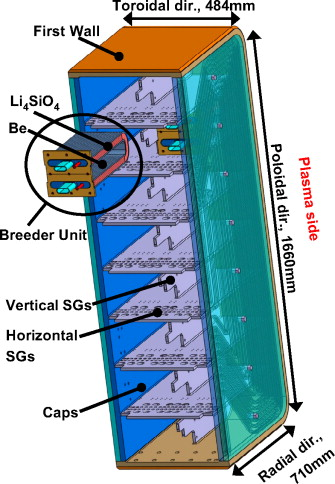
\includegraphics[width=\singleimagewidth]{figures/eu-hcpb-2.png} 
	\caption{breeder units in EU design of HCPB feature breeding zones layered horizontally with coolant above and below.}
	\label{fig:eu-hcpb-2}
\end{figure}


Intrapore natural convection may increase effective conductivity of a medium and has therefore received attention in the engineering field since the 1940s. The problem can be considered as a porous medium analog to the Rayleigh-Benard problem and the solution for a simple duct to be shown next follows similar mathematical constructs.

We consider a duct such that the upper boundary is at $z = H$ and lower boundary at $z=0$, with respective temperatures of $T_0$ and $T_0+\Delta T$. The adverse temperature gradient $\Delta T/H$ will give rise to natural convection under certain circumstances. Assuming that the medium in this duct is homogeneous, isotropic, Darcy's law is valid, and the Boussinesq approximation is valid, the governing equations reduce to
\begin{align}\label{eq:packed-bed-eqns}
\nabla\cdot \vec{v}&= 0 \\
c_a\rho_0\dt{\vec{v}} &= -\nabla P - \frac{\mu}{K}\vec{v} + \rho_f\vec{g} \\
(\rho c)_m\dt{T} + (\rho c_P)_f\vec{v}\cdot\nabla T &= k_m \nabla^2T
\end{align}
where $c_a$ is an acceleration coefficient, unique to porous media. Its definition is described in more detail in Ref.\cite{Nield2013} . Temperature dependence enters density via $\rho_f = \rho_0[1-\beta(T-T_0)]$. $K$ is the permeability of the packed bed, its calculation will be shown later.
%  which for a bed of spherical particles can be found from reduction of the Cozeny-Karman relation to be
% \begin{equation}
% K = \frac{d_p^2 \epsilon^3}{180(1-\epsilon)^2}
% \end{equation}

For any variable with subscript as $\psi_m$, it is calculated as the two-phase average,
\begin{equation}
\psi_m = (1-\epsilon)\psi_s + \epsilon \psi_f
\end{equation}

One solution to \Cref{eq:packed-bed-eqns} is the stagnant, pure-conduction condition,\cite{Nield2013}
\begin{align}
\vec{v}_b &= 0 \\
T_b &= T_0 + \Delta T(1-\frac{z}{H}) \\
P_b &= P_0 - \rho_0 g\left[z + \frac{1}{2}\beta\Delta T\left(\frac{z^2}{H}-2z\right)\right]
\end{align}

Natural convection may be considered an instability in the conduction solution. Therefore we consider the sensitivity of the above to small perturbations. The variables are then
\begin{align}
\vec{v} &= \vec{v}_b + \vec{v}' \\
T &= T_b + T' \\
P &= P_b + P'
\end{align}
which, when inserted back into the conservation equations and higher order perturbation terms are neglected, yield
\begin{align}\label{eq:perturbed}
\nabla\cdot \vec{v}'&= 0 \\
\c_a\rho_0\dt{\vec{v}'} &= -\nabla P' - \frac{\mu}{K}\vec{v}' -\beta\rho_0T'\vec{g} \\
(\rho c)_m\dt{T'} - (\rho c_P)_f\frac{\Delta T}{H}w' &= k_m \nabla^2T'
\end{align}

We next nondimensionalize \Cref{eq:perturbed} with the following dimensionless variables,
\begin{align}
x^* &= \frac{x}{H} \\
t^* &= \frac{\alpha_m t}{\sigma H^2} \\
\vec{v}^* &= \frac{H \vec{v}'}{\alpha_m} \\
T^* &= \frac{T}{\Delta T} \\
P^* &= \frac{K P'}{\mu \alpha_m}
\end{align}
where $\sigma$ is a heat capacity ratio, 
\begin{equation}
\sigma = \frac{(\rho c)_m}{(\rho c_p)_f}
\end{equation}

With nondimensional parameters, we arrive at the following form of nondimensionalized equations
\begin{align}
\nabla\cdot\vec{v}^* &= 0 \label{eq:dimensionless-perturbed-cont}\\
\gamma_a \dt{\vec{v}^*} &= -\nabla P^* -\vec{v}^* + \Ra T^*\vec{k} \label{eq:dimensionless-perturbed-mom} \\ 
\dt{T^*} - w^* &= \nabla^2T^* \label{eq:dimensionless-perturbed-en}
\end{align}
where $\vec{k}$ is the unit vector in the $z$ direction. The dimensionless parameters arising in the momentum equation are
\begin{align}\label{eq:dimensionless-perturbed}
\Ra &= \frac{\rho_0 g \beta K H \Delta T}{\mu \alpha_m} \\
\gamma_a &= \frac{c_a K}{\sigma\Pr_m H^2} \\
\Pr_m &= \frac{\nu_0}{\alpha_m}
\end{align}
$\Ra$ is the Darcian Rayleigh number, differentiated from the standard Rayleigh number by the contribution of permeability, $K$. $\Pr_m$ is the overall Prandtl number of the two-phase medium. And $\gamma_a$ is a dimensionless acceleration coefficient of the fluid.

From \Cref{eq:dimensionless-perturbed-mom}, we see the strength of the coupling between energy and momentum is dependent on the magnitude of $\Ra$; above a critical value, temperature gradients in the medium will induce motion in the fluid.

Nield \& Bejan provide a solution for the set of equations \Cref{eq:dimensionless-perturbed-cont,eq:dimensionless-perturbed-mom,eq:dimensionless-perturbed-en} assuming the acceleration parameter is negligibly small, $\gamma_a = 0$.\cite{Nield2013} The Darcy number, $K/H^2$ is generally quite small and is, in the case of ceramic breeder beds indeed small, and their assumption is applicable. The homogeneous equations form an eigenvalue system for which the eigenvalue is $\Ra$. Ultimately, a stable and real solution is determinable provided that 
\begin{equation}\label{eq:rayleigh-eigen}
\Ra = \frac{(j^2\pi^2 + \omega^2)^2}{\omega^2}
\end{equation}
where $\omega$ is an overall horizontal wavenumber and $j = 1, 2, 3, \dots$.\cite{Nield2013} The minimum of the above occurs when $j = 1$ and $\omega = \pi$ and thus the critical Rayleigh number is $\Ra_c = 4\pi^2 \approx 39.48$. This result suggests that conduction state remains stable for cases of Darcian Rayleigh number less than $4\pi^2$, \textit{i.e.} $\Ra < 39.48$. For Rayleigh numbers larger than this value, convective cells of cellular motion will appear in the porous media fluid.

Combarnous and Bia experimentally studied buoyancy-induced secondary flows through a porous medium in rectangular duct.\cite{Combarnous} They found that in cases of large horizontal to vertical aspect ratios, axial flow did not affect the critical Rayleigh number predicted by linear stability theory. In horizontally-configured solid breeder volumes, aspect ratios are on the order of $A \approx 30$ and thus the critical Rayleigh number defined from perturbation theory, $\Ra < 39.48$, is applicable.

Thus we must finally calculate the Darcian Rayleigh number for a condition such as the European HCPB. Permeability is defined from the relationship to the superficial velocity, viscosity, and pressure drop,
\begin{equation}
\bar{U} = -\frac{K}{\mu}\nabla P
\end{equation}
or
\begin{equation}
K = -\frac{\bar{U}\mu}{\nabla P}
\end{equation}
where the pressure gradient of a spherical-packed bed can be determined from the Cozeny-Karman relation given in \Cref{eq:K-C-pressure}. Therefore, we write
\begin{equation}\label{eq:permeability}
K = \bar{U}\mu\frac{d_p^2}{180 \bar{U} \mu} \frac{\epsilon^3}{(1-\epsilon)^2}
\end{equation}
which reduces to
\begin{equation}
K = \frac{d_p^2}{180} \frac{\epsilon^3}{(1-\epsilon)^2}
\end{equation}

For a well-packed bed, $\epsilon = 0.36$, of \SI{1}{\milli\meter} pebbles, the permeability is found to be $K = \SI{6.33E-10}{\meter\squared}$.

Taking a half-width of the EU HCPB of \SI{1}{\centi\meter} with a temperature gradient of \SI{400}{\kelvin}, we may take fluid properties at an average value across the bed to ultimately find that the Darcian Rayleigh number is $\Ra = \SI{1.23E-5}{}$ which is significantly less than the critical Rayleigh number, $1.23\times 10^{-5} \ll 39.5$. We may therefore conclude that under standard operating conditions of ITER-like solid breeder pebble beds natural convection \textit{will not occur}.

We may also consider the situation when there is no porous medium present in the duct. In the condition of pure helium, standard Rayleigh number may be calculated,
\begin{equation}
\Ra_f = \frac{\rho_0 g \beta H \Delta T}{\mu \alpha}
\end{equation}
which, for helium between two constant temperatures separated by \SI{1}{\centi\meter} results in a Rayleigh number of only $\Ra_f = 4.86$. For Rayleigh-Benard convective cells to form, the critical Rayleigh number is around $\Ra_f = 1000$, which is significantly higher than what we have found. Ultimately, the narrowness of the solid breeder volume prevents buoyant forces from ever overcoming viscous forces in the two-phase form of helium and lithium ceramic.
% However, we may reverse the calculation to determine scenarios of HCPB that would lead to Darcian Rayleigh numbers above the critical value. We need not consider the situation of different temperature gradient across the bed as this parameter is driven by tritium release concerns of the material. Therefore, we will simply consider the permeability value that would lead to natural convection. The permeability exceeding the critical Rayleigh number can therefore be found as $K>Ra_c/C$ where $C = \SI{1.98E4}{\per\meter\squared}$. Permeability is a function of void fraction and diameter, as given in \Cref{eq:permeability}.

% Under the current consideration, if we consider a well-packed bed of void fraction $\epsilon = 0.36$, it would require pebbles of diameter $d_p = \SI{2}{\meter}$ in order to exceed the critical Darcian Rayleigh number. Likewise, for pebbles of \SI{1}{\milli\meter}, the void fraction would have to increase to a virtually empty duct, $\ep = 0.998$.